%-----------------------------------------------------------------------------
%
%               Template for sigplanconf LaTeX Class
%
% Name:         sigplanconf-template.tex
%
% Purpose:      A template for sigplanconf.cls, which is a LaTeX 2e class
%               file for SIGPLAN conference proceedings.
%
% Guide:        Refer to "Author's Guide to the ACM SIGPLAN Class,"
%               sigplanconf-guide.pdf
%
% Author:       Paul C. Anagnostopoulos
%               Windfall Software
%               978 371-2316
%               paul@windfall.com
%
% Created:      15 February 2005
%
%-----------------------------------------------------------------------------


\documentclass[preprint]{sigplanconf}

% The following \documentclass options may be useful:

% preprint      Remove this option only once the paper is in final form.
% 10pt          To set in 10-point type instead of 9-point.
% 11pt          To set in 11-point type instead of 9-point.
% numbers       To obtain numeric citation style instead of author/year.

\usepackage[utf8]{inputenc}
\usepackage[T1]{fontenc}
\usepackage{listings}
\usepackage[rgb,dvipsnames]{xcolor}
\usepackage{hyperref}
\usepackage{graphics}
\usepackage{array} % tables
\usepackage{afterpage} % figures
\usepackage{float} % figures
\usepackage{paralist} % figures
\usepackage[shortcuts]{extdash} % figures
\usepackage{todonotes}
\usepackage{textcomp}
\usepackage{ marvosym }
\usepackage{dirtree}
% \usepackage{lmodern}
\usepackage{multirow,tabularx}
\usepackage{ctable}
\usepackage{relsize}
\usepackage{amsmath,amssymb}
\usepackage{algorithm}
\usepackage{algpseudocode}
\usepackage{pifont}
\usepackage{amsthm}
\usepackage{siunitx}
 \sisetup{
    binary-units,
    detect-all,
    free-standing-units,
    space-before-unit,
    use-xspace,
    unit-optional-argument,
    parse-units = false,
  }
%\usepackage[scaled=0.9]{inconsolata}
\usepackage[scaled=0.85]{beramono}
\usepackage[final]{microtype}
\microtypesetup{stretch=9,shrink=15,step=3,letterspace=50}
% % Disable single lines at the start of a paragraph (Schusterjungen)
% \clubpenalty = 10000
% % Disable single lines at the end of a paragraph (Hurenkinder)
% \widowpenalty = 10000 
% \displaywidowpenalty = 10000 % formulas

\usepackage[pass,letterpaper]{geometry}

\usepackage{balance}
%\usepackage{subcaption}
\usepackage{subfig}
\usepackage{wrapfig}

\newcommand{\cL}{{\cal L}}

\lstset{
language=Ruby,
% backgroundcolor=\color[rgb]{0.95, 0.95, 0.95},
tabsize=2,
rulecolor=,
basicstyle=\ttfamily,
upquote=true,
% aboveskip={1.5\baselineskip},
columns=fullflexible,
% columns=fixed,
showstringspaces=false,
extendedchars=true,
breaklines=true,
prebreak = \raisebox{0ex}[0ex][0ex]{\ensuremath{\hookleftarrow}},
% frame=single,
showtabs=false,
showspaces=false,
showstringspaces=false,
% identifierstyle=\ttfamily,
keywordstyle=\color[rgb]{1.0,0,0},
keywordstyle=[1]\color[rgb]{0,0,0.75},
keywordstyle=[2]\color[rgb]{0.5,0.0,0.0},
keywordstyle=[3]\color[rgb]{0.127,0.427,0.514},
keywordstyle=[4]\color[rgb]{0.4,0.4,0.4},
commentstyle=\color[rgb]{0,0,0},
stringstyle=\color[rgb]{0.639,0.082,0.082},
morekeywords={self, proceed},
%numbers=left,%
numbersep=5pt,%
numberstyle=\tiny\color{gray},%
emphstyle=\bfseries,%
breaklines=true,
breakatwhitespace=true,%
escapechar=`,
}
\lstset{escapeinside={<@}{@>}}

\begin{document}

\special{papersize=8.5in,11in}
\setlength{\pdfpageheight}{\paperheight}
\setlength{\pdfpagewidth}{\paperwidth}

\conferenceinfo{ARRAY '16}{Month d--d, 20yy, Malaga, Spain}
\copyrightyear{2016}
\copyrightdata{978-1-nnnn-nnnn-n/yy/mm}
\copyrightdoi{nnnnnnn.nnnnnnn}

% Uncomment the publication rights you want to use.
%\publicationrights{transferred}
\publicationrights{licensed}     % this is the default
%\publicationrights{author-pays}
\toappear{}

\titlebanner{Submitted for review to ARRAY 2016}        % These are ignored unless
\preprintfooter{Ikra: Object-oriented GPGPU Programming in Ruby with CUDA}   % 'preprint' option specified.

\title{Ikra: Object-oriented GPGPU Programming \\ in Ruby with CUDA}
%\title{A Layer-based Approach to Hierarchical Dynamically-scoped Class Extensions}

\subtitle{Research Paper}

\newcommand\Mark[1]{\textsuperscript#1}  
\authorinfo{Matthias Springer\and Hidehiko Masuhara}
           {Department of Mathematical and Computing Sciences, Tokyo Institute of Technology, Japan}
           {matthias.springer@acm.org \and masuhara@acm.org}     
\maketitle

\setcitestyle{square}

\captionsetup{labelfont=bf}

\begin{abstract}
This paper presents implementation and optimization techniques to support objects in Ikra, an array-based parallel extension to Ruby with a just-in-time compiler. The high-level goal of Ikra is to allow developers to exploit GPU-based high-performance computing without having to be familiar with intricate details of the underlying GPU infrastructure and CUDA.

Ikra supports dynamically-typed object-oriented programming in Ruby and performs a number of optimizations. To reduce thread divergence, Ikra reorders jobs in the base array based on type information. To facilitate memory coalescing, Ikra stores objects in a fields-of-arrays representation (columnar object layout). To support a larger subset of Ruby, polymorphic method calls are allowed in parallel sections and compiled to conditional branches. Cascaded parallel sections can be arbitrarily interleaved with non-parallel sections, are executed symbolically, and are merged into one kernel and executed upon accessing the result.

%Ikra analyzes parallel sections in the form of array operations (e.g., \texttt{map}, \texttt{select}, or \texttt{each}), performs type inference upon invocation, and generates a CUDA kernel. To reduce thread divergence, Ikra reorders the base array based on the type information, which is useful for programs that were designed in an object-oriented way. Objects are represented as columns, giving rise to memory coalescing. Although programmers are advised to write statically-typed Ruby code for performance reasons, Ikra can generate CUDA code for expressions that can be one of multiple types using class tags.
\end{abstract}

\category{D.1.3}{Concurrent Programming}{Parallel Programming}
\category{D.3.4}{Processors}{Code generation, Compilers}

% general terms are not compulsory anymore,
% you may leave them out
%\terms
%term1, term2

\keywords
GPGPU, CUDA, Ruby, object-oriented programming

\section{Introduction}
With the availability and affordability of powerful GPUs, general purpose computing on graphics processing units (GPGPU) is becoming more and more popular in high-performance computing. Nowadays, many supercomputers rely on GPUs as main processing units, because they allow for massively parallel execution of algorithms or simulations with thousands of threads per GPU. However, GPU programming differs from traditional CPU programming, mostly because of architectural differences.

The goal of the Ikra project is to make GPU programming available to researchers who are not familiar with the details of GPUs and their programming languages. Ikra is a library for Ruby that translates parallel sections to CUDA code and executes them in parallel on GPUs. It extends our previous work~\cite{Masuhara:2012:DER:2237887.2237888} with a just-in-time approach to allow for a larger number of optimizations and tighter integration with Ruby. We target the Ruby programming language because it provides powerful mechanisms for embedding DSLs in the language, which will be useful for later experiments.

\section{Example: Actor-based Traffic Simulation}
A simple actor-based traffic simulation will serve as a running example in this paper. The basic idea is to simulate the behavior of a number of actors~\cite{Helbing2012} (e.g., cars, buses, pedestrians, etc.), given a street network as a directed graph (Figure~\ref{fig:running_example}) in adjacency list representation. Every actor is located on one street. Every street has a \emph{length} attribute and every actor has a \emph{progress} attribute representing the distance from the beginning of the street. Once these two attributes have the same value, the actor reached an intersection and should be moved to a different street (or make a U-turn if there is no other neighboring street).

\begin{figure}[!htp]
    \centering
    \subfloat[Actual street network (map)]{{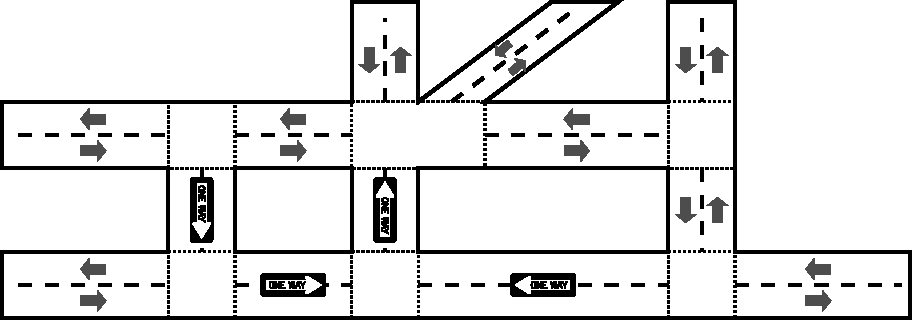
\includegraphics[width=\columnwidth]{running_example.pdf} }}%
    
    \subfloat[Street network as directed graph]{{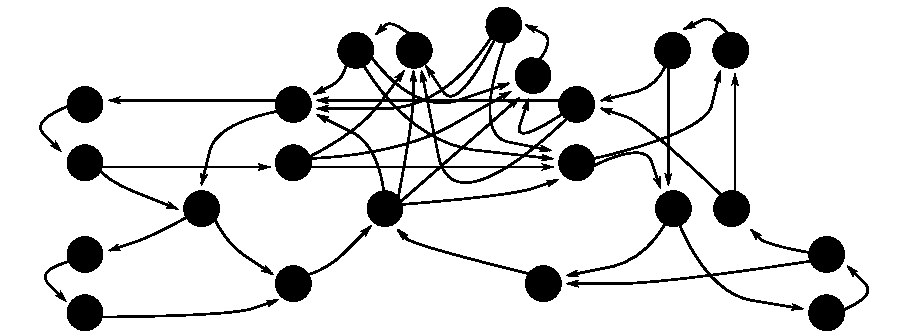
\includegraphics[width=\columnwidth]{running_example_graph.pdf} }}%
    \caption{Example: Street Network for Traffic Simulation}
    \label{fig:running_example}%
\end{figure}

A car moves at a constant speed of $\min(M_c, M_s)$, where $M_c$ is the maximum velocity of the car and $M_s$ is the maximum speed allowed on the current street. A pedestrian moves at a random speed between $-2$~mph and $4$~mph, i.e., a pedestrian can make negative progress. This is how we model strolling pedestrians. Furthermore, depending on their type, the progress of actors might be affected by weather conditions. For example, cars slow down if the weather conditions are bad, whereas pedestrians are not affected by weather.

\paragraph{Data Structure}
The street network and the actors are designed in an object-oriented way. Figure~\ref{fig:running_example_classes} shows the class organization of the traffic simulation. \texttt{Car} and \texttt{Pedestrian} are subclasses of \texttt{Actor} and provide their own \texttt{move} methods which will be invoked for every tick of the simulation. 

\begin{figure}[!htp]
    \centering
    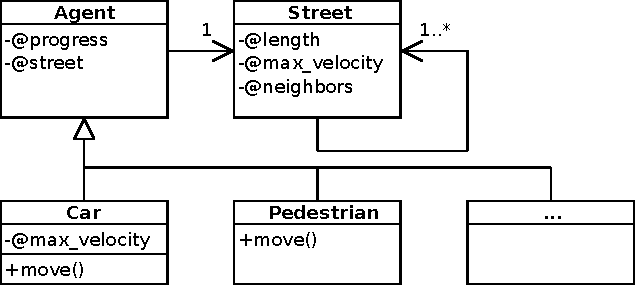
\includegraphics[width=0.8\columnwidth]{class_diagram_running_ex.pdf}
    \caption{Class Diagram for Traffic Simulation}
    \label{fig:running_example_classes}
\end{figure}

\paragraph{Main Simulation Loop}
The following code snippet contains the main simulation functionality. The method \texttt{pmap} designates a parallel section. Its parameter \texttt{ticks} determines how often the entire \texttt{peach} statement should be executed and is equivalent to wrapping the \texttt{peach} statement in a loop that executes it \texttt{ticks} times\footnote{There are currently certain limitations for loop nesting. See Section~\ref{sec:nested_loops} for more details.}.

\begin{lstlisting}
actors = [...]
ticks = 1000
weather = Weather::Rainy

actors.peach(ticks) <@\textbf{do}@> |actor|
    actor.move(weather)
<@\textbf{end}@>
\end{lstlisting}

Every \emph{tick} of the simulation progresses the current time by a certain constant value and actors are required to update their progress and street attributes accordingly.

\section{Architecture}
Ikra is a library for Ruby. It adds functionality to arrays to execute \texttt{map}, \texttt{select} and \texttt{each} operations in parallel. Programmers can \emph{require} Ikra in Ruby files, upon which new parallel versions of array operations are available (e.g., \texttt{pmap}). These parallel array operations take a block as an argument, designate the only parts of a Ruby programs that are parallelized using Ikra, and are executed symbolically. Parallel array operations (except for \texttt{peach}) can be cascaded and are executed only if the result is actually accessed. The default behavior is to spawn one thread per array element, which is why all these computations must be independent of each other. 

\subsection{Compilation Process}
Figure~\ref{fig:overview_arch} gives a high-level overview of Ikra's compilation process. Upon invocation of a parallel section, Ikra acquires the source code of the parallel block, generates an abstract syntax tree (AST), and infers the type of all expressions. As a result, the type of every local and instance variable is known. In the best case, the type of an expression is monomorphic and primitive, but Ikra also supports arbitrary Ruby classes as types, as well as polymorphic types (see Section~\ref{sec:polymorphic}). The type inferer traverses invoked methods in a may-point-to fashion\footnote{Methods of all possible receiver types are taken into account.}. Based on the type-annotated AST, Ikra generates CUDA kernel code and boilerplate code for kernel invocation, and compiles the CUDA code using the nVidia CUDA toolchain. The result is a shared library which is loaded via Ruby's foreign function interface. Before kernel invocation, the base array and lexical variables along with all reachable objects (via instance variables) are transferred to the GPU's global memory. After kernel invocation, all changed objects and the result of the parallel section (if applicable) are written back to Ruby.

\begin{figure}[!tp]
    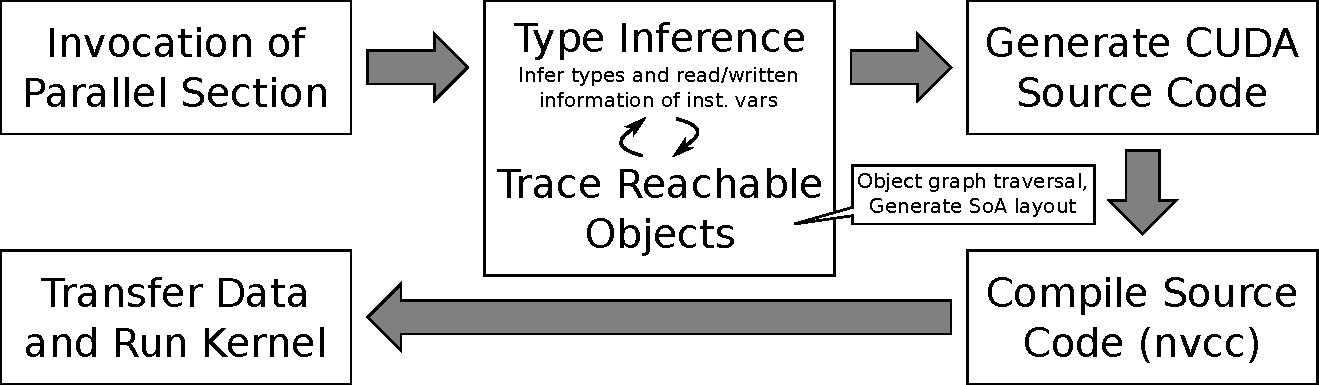
\includegraphics[width=\columnwidth]{high_level_arch.pdf}
    \caption{Overview of Ikra's Architecture}
    \label{fig:overview_arch}
\end{figure}

Ikra performs \emph{kernel fusion}~\cite{Wu:2012:KWA:2457472.2457490, Wahib:2014:SKF:2683593.2683615}, i.e., cascaded parallel operations are merged into a single CUDA kernel to avoid writing intermediate results to the global memory. Instead, they can be kept in registers. The process of merging two parallel blocks is not relevant in the scope of this paper and omitted.

\subsection{Integration in Ruby}
In contrast to some other projects, Ikra transforms Ruby code to CUDA code while the Ruby program is running (just-in-time compilation). Therefore, Ikra can determine the types of variables that are passed into parallel sections at runtime instead of doing a dataflow analysis of the entire program. This is not only faster but also more accurate in the light of reflection and metaprogramming, which is allowed outside of parallel sections but not inside them.

Two different kinds of variables can be used inside a parallel section: iterator variables and lexical variables\footnote{Instance variables can be used when calling an instance method.}. In the main loop of the traffic simulation example, \texttt{actor} is an iterator variable and \texttt{weather} is a lexical variable. The types of these variables are used as the basis for type inference of the remaining parallel section.

Programmers can use not only primitive objects (\texttt{Fixnum}, \texttt{Float}, etc.) but also objects which are instances of Ruby classes inside parallel sections, allowing for object-oriented modelling of the problem (e.g., a traffic simulation). Consequently, a graph of \emph{reachable} (connected) objects must be transferred to the GPU. The \emph{object tracer} is responsible for determining which objects should be copied to the GPU's global memory (see Section~\ref{sec:impl_tracer}).

After kernel execution, changed local variables and instance variables are copied back to the Ruby side (see Section~\ref{sec:impl_copyback}).


\section{Implementation and Optimizations}
In this section, we give an overview of some interesting aspects of Ikra's implementation.

\subsection{Job Reordering}
Before kernel invocation, Ikra analyzes all elements in the base array and reorders them according to their type. This is useful to avoid \emph{thread divergence}, which can penalize performance when running programs on GPUs.

\paragraph{Thread Divergence}
In contrast to most CPU-based systems\footnote{There are CPU extensions for SIMD computations, e.g., SSE.}, GPU-based systems are SIMD (single instruction, multiple data) systems. A GPU consists of a number of streaming multiprocessors. Such a processor has a single control unit that fetches and decodes instructions, but multiple arithmetic logic units (ALUs). Therefore, every instruction is executed in parallel on multiple chunks of data. Every ALU corresponds to one thread, but all threads that are executing on the same streaming multiprocessor must follow the same control flow. In case two threads take a different branch, their execution is serialized until the control flow merges again. Consequently, jobs should be threads/jobs should be mapped to streaming multiprocessors in such a way that the control flow is unlikely to divergence among one such thread group (threads executing on one streaming multiprocessor).

In CUDA, such a thread group is called \emph{warp} and has a size of 32. There is no explicit interface to allocate threads to warps, but CUDA programmers try to write their programs in such a way that each consecutive group of 32 threads follows the same control flow.

\paragraph{Thread Allocation}
Ikra tries to avoid thread divergence by allocating jobs to warps automatically based on type information. Before kernel invocation, Ikra generates a \emph{job reordering array}, such that the base array is sorted according the elements' types (Figure~\ref{fig:ex_job_reorder}). Ikra does not actually change the order elements in the base array to ensure that other parts of the program outside of the parallel section are not affected.

\begin{figure}[!htp]
    \centering
    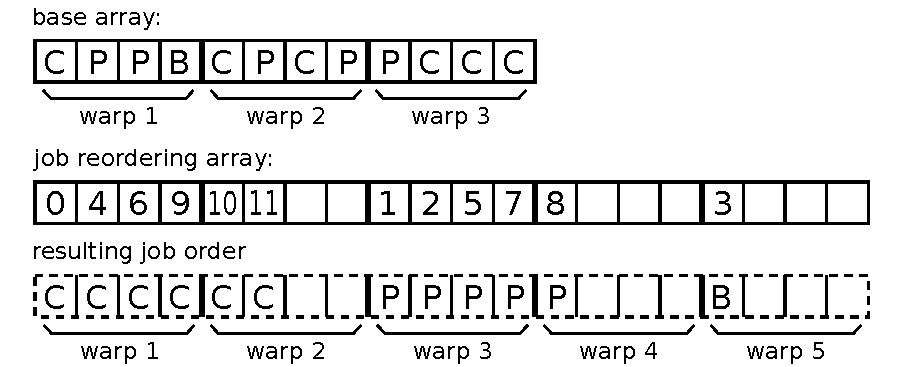
\includegraphics[width=\columnwidth]{reorder_example.pdf}
    \caption{Example: Job Reordering. The first row is the original job order, the second row is the job reordering array, and the third row shows the resulting job order (warp size 4).}
    \label{fig:ex_job_reorder}
\end{figure}

During job reordering the number of threads can increase as shown in Figure~\ref{fig:ex_job_reorder}. Jobs are reordered in such a way that no two elements of different types are allocated in the same warp. If the number of jobs of a particular type is not a multiple of the warp size, the last warp will not be filled up entirely, but some threads will not have a job, i.e., they are not \emph{no operation} threads. This might seem like a waste of computing power, but we expect the number of different types to be small (3 in this example).

The job reordering array can be computed in linear time by scanning all elements of the base array twice. The pseudo code in Algorithm~1 is similar to counting sort and bucket sort~\cite{Corwin:2004:SLT:1040231.1040257}. It generates one array of indices per type (class) and concatenates these arrays, making sure that every new array starts at a multiple of the warp size $W$.

\begin{algorithm}
\caption{Job Reordering}
\label{CHalgorithm}
\begin{algorithmic}[1]
\Procedure{ReorderingArray}{base, W}
\State $\mathit{types} \gets$ Hash.new \hfill \textcolor{gray}{\textit{default value:} Array.new}
\ForAll {$(\mathit{el}, \mathit{idx}) \in \mathit{base}$}
    \State $\mathit{types}[\mathit{el}.\mbox{class}].\mbox{add}(\mathit{idx})$
\EndFor
\State $\mathit{result} \gets$ Array.new$(\sum_{\mathit{arr} \in \mathit{types}.\mathit{values}} \lceil |\mathit{arr}| / W \rceil * W)$
\State $\mathit{next} \gets 0$
\ForAll {$\mathit{arr} \in \mathit{types}.\mbox{values}$}
    \ForAll {$\mathit{idx} \in \mathit{arr}$}
        \State $\mathit{result}[\mathit{next}] = \mathit{idx}$
        \State $\mathit{next} \gets \mathit{next} + 1$
    \EndFor
    \State $\mathit{next} \gets \lceil \mathit{next} / W \rceil * W$
\EndFor
\State \Return $\mathit{result}$
\EndProcedure
\end{algorithmic}
\end{algorithm}


\subsection{Columnar Object Layout}
In traditional programming languages and virtual machines, objects are typically represented row-wise, i.e., every object is a contiguous chunk of data in the memory. However, it is common practice in GPU programming to work with multiple arrays of structure fields instead of one array of structures.

\paragraph{Memory Coalescing}
Global memory is one of the main bottlenecks of GPUs. One approach is to aim for memory access patterns where memory that is accessed in parallel by a number of threads is spatially local. Such memory accesses can be coalesced, i.e., the GPU can process such accesses in a single request, alleviating the global memory bottleneck.

Since a GPU is a SIMD system, all threads within a warp have to execute the same instruction at a time. Consequently, if one thread accesses an instance variable, then all other threads within the same warp access the same instance variable (or block because of thread divergence), probably in a different object. In this situation, a columnar object layout is superior to a row-based object layout, because parallel accesses to the same instance variable are more likely to be spatially local (Figure~\ref{fig:ex_obj_layout}).

\begin{figure}[!htp]
    \centering
    \subfloat[Row-based Layout (uncoalesced)]{{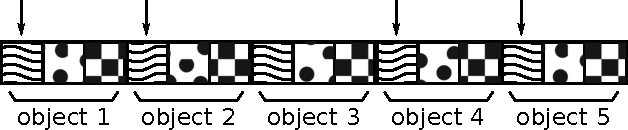
\includegraphics[width=0.75\columnwidth]{column_access_1.pdf} }}%
    
    \subfloat[Column-based Layout (maybe coalesced)]{{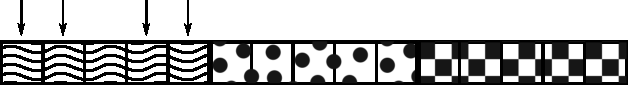
\includegraphics[width=0.75\columnwidth]{column_access_2.pdf} }}%
    \caption{Example: Row-based and Column-based Object Layout. Boxes represent instance variables. Arrows indicate parallel access.}
    \label{fig:ex_obj_layout}%
\end{figure}

\paragraph{Generating Columns}
In the following, we present a first approach for representing objects as columns. For the moment, we assume that all source code is statically typed and the types of all expressions and variables were inferred successfully. This approach will be extended in the light of polymorphic expressions in the next section.

After running the object tracer, we know which objects should be transferred to the GPU. These objects are processed as follows.
\begin{enumerate}
    \item Group objects by their classes $c$, resulting in arrays $O_c$.
    \item Assign an ID to every object for all $O_c$, starting from $0$ in every $O_c$, IDs being consecutive. This results in a hash map $H_c$ mapping objects to class-specific IDs.
    \item For every instance variable $v$ of every class $c$, create an array (column) $A_{c,v}$ of size $m + 1$, where $m$ is the maximum ID in $O_c$. The base type of the array is the type of the instance variable if it is primitive, or \texttt{int} otherwise (referencing other non-primitive objects via their IDs).
    \item For every object $o$ with class $c$ and ID $H_c[o]$, store every instance variable $v$ in the corresponding column slot $A_{c, v}[H_c[o]]$. If the instance variable is non-primitive, look up its ID and store it.
\end{enumerate}

Note that after this transformation, the base type of the base array that is passed to the kernel, is \texttt{int} and contains object IDs if it contains non-primitive objects.

In our implementation, the object tracer is combined with the column generator. A pseudo code implementation which was also used for benchmarks is shown in Section~\ref{sec:appendix_obj_tracer}.

\paragraph{Source Code Transformation}
Since objects are now represented as fields of arrays, Ikra must generate different source code for reading from or writing to instance variables. We continue to assume that the type of all expressions and variables is known unambiguously. Moreover, we do not consider generating new objects at this time (see Section~\ref{sec:gen_new_obj}).

In the following, we consider reading/writing instance variables of an object and calling methods on an object, where the object is identified by its type $c$ and its ID $i$. Whenever objects are passed around, Ikra actually generates source code that passes their IDs around. Passing type information is not necessary, because we assume that we know the type of every expression and variable\footnote{We consider subclasses to be an entirely different type in this section.}.

Reading an instance variable $v$ of object $o$ with type $c$ and ID $i$ translates to reading the column $A_{c,v}[i]$. Writing an instance variable translates to writing into the same column at the same position.

Every instance method is translated to a device function, where the type $c$ is mangled into its name and the first parameter has type \texttt{int} and represents the ID of \texttt{self} object. Whenever Ikra encounters a method call during code translation, it determines the receiver's type and generates a call to the appropriate device function.

\paragraph{Representation of Arrays}
The previously-described mechanism for columnar objects works well with equally-sized objects, but not for variable-sized objects such as arrays. For example, the instance variable \texttt{@neighbors} of class \texttt{Street} is an array of streets.

Ikra effectively represents such $n:m$ relationships as join tables~\cite{Garcia-Molina:2008:DSC:1450931} that are \emph{collapsed}. Such a table is sorted by object IDs for $n$. Furthermore, the $n$ column is not stored as a full column but as RLE tuples~\cite{Abadi:2006:ICE:1142473.1142548} consisting of an implicit ID for $n$, a start offset into the $m$ column, and a length value, distributed among multiple columns. RLE tuples are a well-known optimization in column databases.

\begin{figure}[!htp]
    \centering
    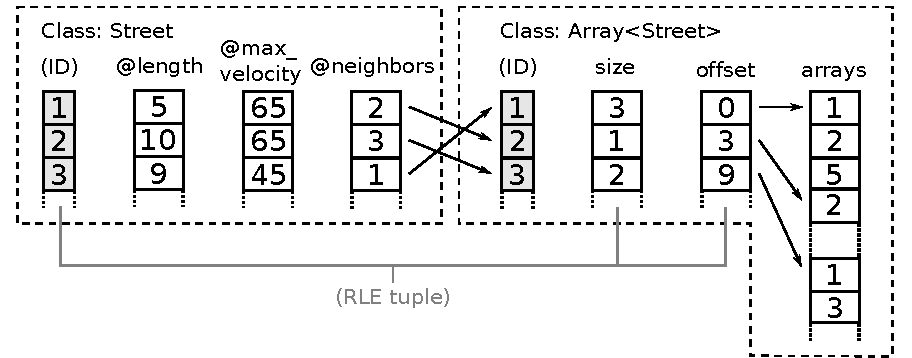
\includegraphics[width=\columnwidth]{column_access.pdf}
    \caption{Example: Array Representation for \texttt{@neighbors} ($n:m$ relationship). $(\texttt{Street.ID}, \texttt{Array.offset}, \texttt{Array.size})$ is an RLE tuple~\cite{Abadi:2006:ICE:1142473.1142548}.}
    \label{fig:array_repr}
\end{figure}

From an implementation point of view, an array is an ordinary object with an offset and a size attribute. The offset attribute points into a single large array containing the contents of all arrays. This layout might change in future versions of Ikra (see Section~\ref{sec:gen_new_obj}).

%One approach to alleviate that problem is to aim for a high occupancy to hide memory latency, i.e., running a high number of threads, such that the GPU can switch execution to another warp while the current thread is blocking. Another optimization is to aim for coalesced mem

\subsection{Dynamically-typed Expressions}
\label{sec:polymorphic}
In contrast to CUDA, Ruby is a dynamically-typed programming language. One of the goals of the Ikra project is to allow programmers to write Ruby code in a \emph{natural} way, i.e., programmers should be able to write the same source code that they would write in a standard Ruby environment. For this reason, Ikra should also support Ruby expression whose types cannot be inferred unambiguously at translation time.

Ikra embeds dynamic types into CUDA's static type system by generating explicit type dispatch statements at method call sites based on type tags~\cite{Abadi:1989:DTS:75277.75296} for receivers whose types cannot be inferred unambiguously. From a perspective of object-oriented design, this looks as if every object has a \emph{type} instance variable.

\paragraph{Class Tags}
To support dynamically-typed expressions, we extend the idea of class-specific object IDs as follows. The following mechanism is applied only if the type of an expression or variable cannot be uniquely inferred. Otherwise, the previously described (non-extended) mechanism is applied. 

Whenever an object ID was previously used, we now use a tuple of object ID and \emph{class tag}. A class tag is a unique \texttt{int} identifier for a certain class. Class tags are used for object references and for method calls. A Ruby variable is now represented by two CUDA \texttt{int} variables: one for the class tag and one for the object ID. Similarly, when passing an object as an argument, the same two arguments are passed in the generated CUDA code.

Before dispatching to a method, the generated CUDA code determines the type of the receiver in a switch statement to select the corresponding instance method. In the following example, two arrays (actor tags and actor IDs) are passed to the kernel function. The device function representing the block invokes the correct instance method.

\lstset{language=C++}
\begin{lstlisting}
<@\textbf{\_\_global\_\_ void}@> kernel(<@\textbf{int}@> *jobs, <@\textbf{int}@> *actor_tag, <@\textbf{int}@> *actor_id, <@\textbf{int}@> weather)
{
  <@\textbf{int}@> tid = blockIdx.x * blockDim.x + threadIdx.x;
  block(actor_tag[jobs[id]], actor_id[jobs[id]], weather);
}

<@\textbf{\_\_device\_\_ void}@> block(<@\textbf{int}@> actor_tag, <@\textbf{int}@> actor_id, <@\textbf{int}@> weather)
{
  <@\textbf{for}@> (<@\textbf{int}@> i = 0; i <= ticks; i++)
  {
    <@\textbf{switch}@> (actor_tag)
    {
      <@\textbf{case}@> TAG_Car:
        method_Car_move(actor_id, weather);
        <@\textbf{break}@>;
      <@\textbf{case}@> TAG_Pedestrian:
        method_Pedestrian_move(actor_id, weather);
        <@\textbf{break}@>;
      <@\textbf{default}@>:
        <@\textit{/* same mechanism to dispatch to method\_missing */}@>
    }
  }
}
\end{lstlisting}

\paragraph{Object Layout}
In the light of class tags, we extend the columnar object layout as follows. If Ikra cannot infer the type of an instance variable unambiguously, two columns are created for that instance variable: one for the class tag and one for the object ID.

\paragraph{Polymorphism}
In terms of type inference, subclasses are treated as entirely different types instead of subtypes. For example, if type inference determines that the type of a variable can be \texttt{Car} or \texttt{Pedestrian}, the type of that variable is the set $\{\texttt{Car}, \texttt{Pedestrian}\}$ instead of \texttt{Actor}. In this case, the type dispatch statements for a method call contains can handle only \texttt{Car} and \texttt{Pedestrian}, but not, for example, \texttt{Bus}, which is also a subclass of \texttt{Actor}. If a method is only implemented in a superclass (e.g., \texttt{Actor}), but not in the receiver's class itself (e.g., \texttt{Car}), the generated code can dispatch to that method directly; that case can be detected at translation time. In addition to the object ID of the \texttt{self} (receiver) object, its class tag is also passed as an argument during method calls.

Instance variables are stored together with the first class in the superclass hierarchy, in which they were used for the first time. For example, \texttt{@street} is stored as a column of class \texttt{Actor}. Subclasses and superclass share the same IDs. If an object is an instance of a different subclass, the corresponding column values are \emph{null} values~\cite{Mattis:2015:COI:2814228.2814230}. For example, if object 15 is a \texttt{Pedestrian}, then $A_{\texttt{Car}, \texttt{@max\_velocity}}[15]$ is null.

\subsection{Read/write Analysis for Instance Variables}
\label{sec:impl_copyback}
As part of type inference, Ikra analyzes if an instance variable is read and/or written. Only instance variables that are read or written are transferred to the GPU. Only instance variables that are written are transferred back to the Ruby side directly after kernel invocation. Ikra performs a may-be-read/may-be-written analysis, which can have false positives in case the type of an expression cannot be determined accurately. Ikra does not copy single instance variable values, but entire columns.

\subsection{Object Tracer}
\label{sec:impl_tracer}
The object tracer is responsible for generating a list of objects that must be transferred to the GPU before kernel invocation. It starts with a set of root objects: all elements of the base array and lexical variables. Then, it traverses the object graph by following all instance variables. However, an instance variable value is visited only if that variable is read or written inside the parallel section. The entire process of tracing the object graph and assigning unique object IDs is similar to the \emph{system tracer} component in Smalltalk~\cite{Krasner:1983:SBH:226}.

\section{Microbenchmarks}
To evaluate our optimizations, we conducted a series of microbenchmarks using the traffic simulation example\footnote{\texttt{git@github.com:matthias-springer/array2016-paper.git}}. We ran benchmarks on the Tsubame supercomputer\footnote{\url{http://tsubame.gsic.titech.ac.jp/}} on a \emph{thin} compute node with two Intel Xeon X5670 CPUs (2.93~GHz $\times$ 6 cores each), 54~GB RAM, and an nVidia Tesla K20Xm GPU, running Linux \texttt{3.0.76-0.11-default x86\_64}, CUDA 7.0.27, and Ruby 1.9.3p448.

We simulated 1,000,000 iterations of a random street network with 500 streets and random vertex out-degrees between 1 and 10, 4096 cars, and 16384 pedestrians. All benchmark running times are average values of 5 runs\footnote{GPU running times showed a very low standard deviation.} using the same random scenario.

\paragraph{Kernel Execution}
Figure~\ref{fig:bench_kernel} shows the kernel running time of the traffic simulation in various configurations. Figure~\ref{fig:bench_kernel}a shows the running time with a columnar object layout, which is around 30\% faster than the row-based layout in Figure~\ref{fig:bench_kernel}b.

\begin{figure}[!htp]
    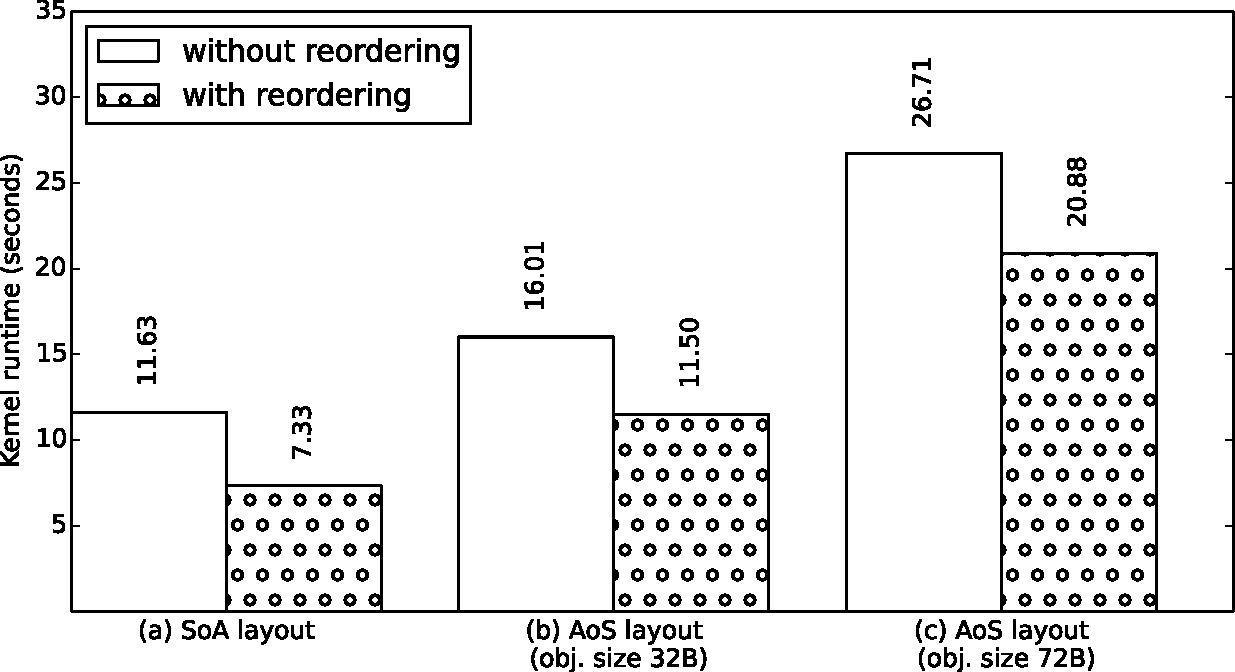
\includegraphics[width=0.95\columnwidth]{bench_1.pdf}
    \centering
    \caption{Kernel Running Time for Traffic Simulation (CUDA)}
    \label{fig:bench_kernel}
\end{figure}

The objects involved in this example are quite small. Actors are represented by 32-byte structs (three instance variables and class tag) in row-based layout, or three 4-byte columns (class tag is passed as an argument) in a columnar layout, respectively. The GPU's L1 cache is 48~KB, with a cache line size of 128~bytes. To analyze the effect of caching, we ran the row-based benchmark with artificially enlarged object sizes (10/5 additional instance variables for actors/streets, resulting in an object size of 72~bytes/32~bytes, respectively; Figure~\ref{fig:bench_kernel}c). This configuration is interesting because the example code accesses all instance variables of an actor subsequently, diminishing the advantage of a column-based layout, because the entire object (and three subsequent objects) can be held in cache (prefetching). A columnar object layout is around 60\% faster compared to this configuration.

\paragraph{Job Reordering}
Figure~\ref{fig:job_reorder_arr} shows the running time for generating the job reordering array (warp size 32). This is currently done in the Ruby interpreter but could be moved to the GPU side in future versions. The running time increases linearly with the number of elements in the base array. Changing the number of types (classes) has only a small effect on the running time. We assume that this number is much smaller than the number of elements. For the traffic simulation example, the running time for generating the job reordering array is neglectable.

\begin{figure}[!htp]
    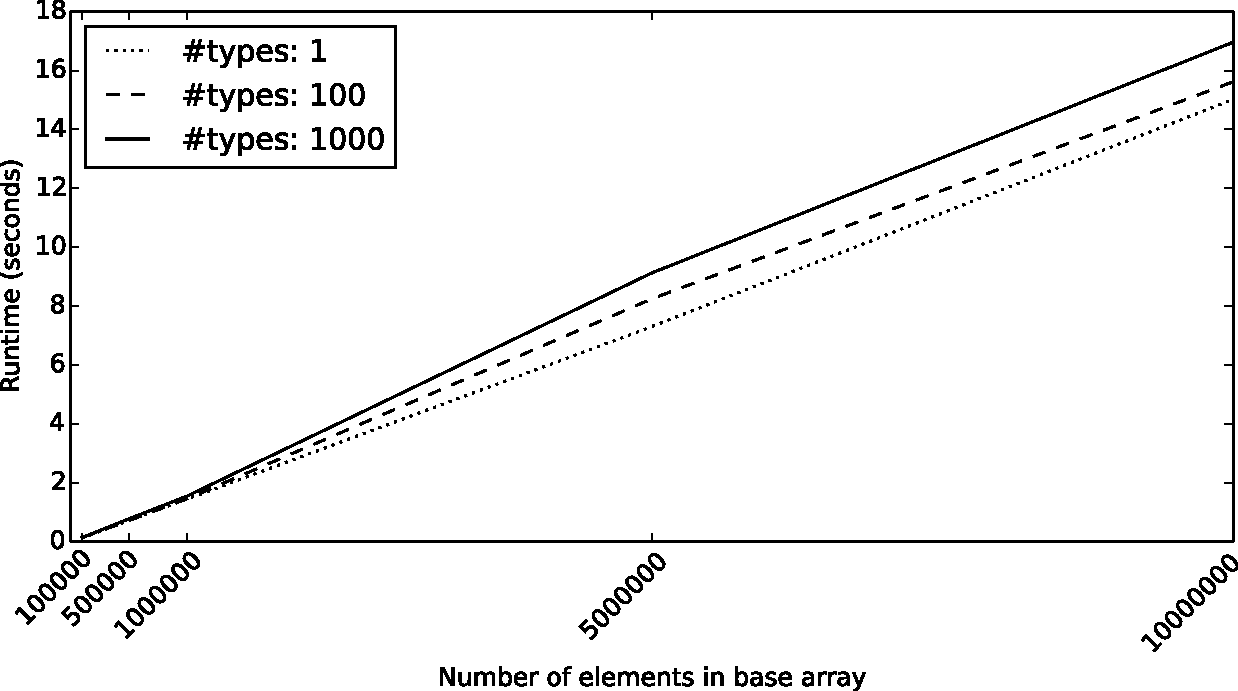
\includegraphics[width=0.9\columnwidth]{plot_reorder.pdf}
    \centering
    \caption{Running Time for Generating Job Reordering Array (Ruby)}
    \label{fig:job_reorder_arr}
\end{figure}

\paragraph{Tracing Object and Generating Columns}
Figure~\ref{fig:tracing} shows the running time for tracing objects and generating columns (Algorithm~2) for the traffic simulation example. For the number of actors/streets that were used in the kernel benchmarks, the running time is neglectable. Moreover, in future plans for Ikra we want to perform this step only once and reuse data that was already processed and moved to the GPU earlier (see Section~\ref{sec:minimizing_dtr}).

\begin{figure}[!htp]
    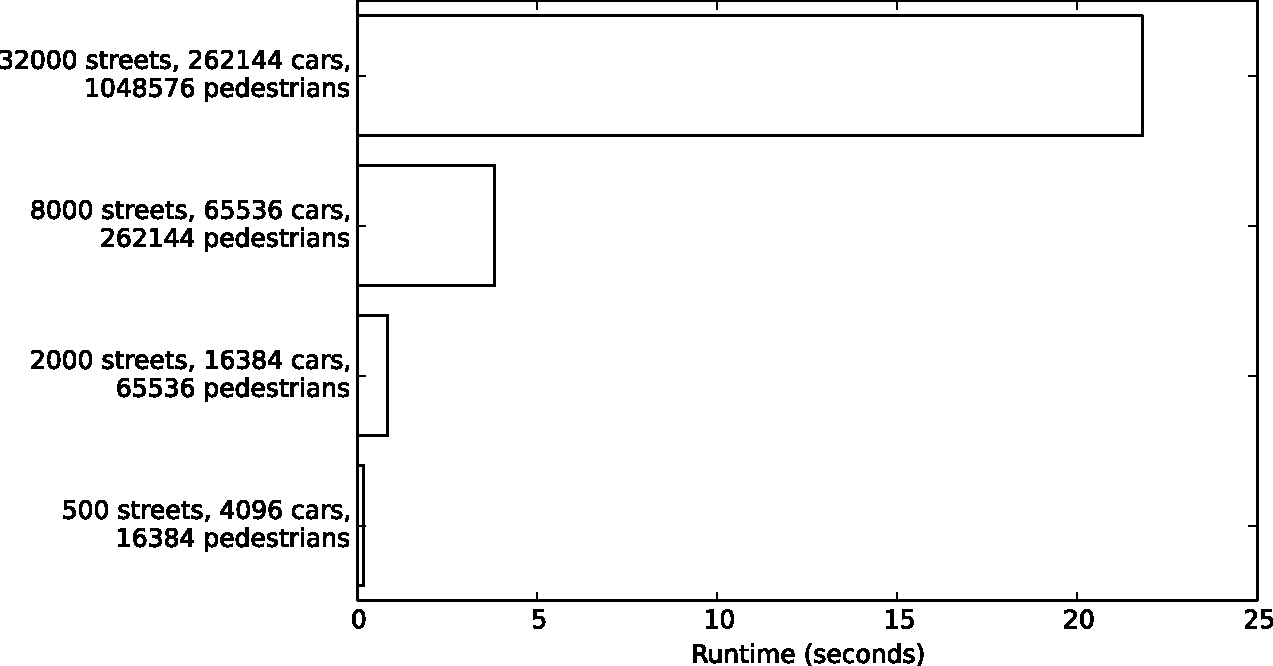
\includegraphics[width=\columnwidth]{obj_tracer.pdf}
    \centering
    \caption{Running Time for Tracing Objects and Generating Columns (Ruby)}
    \label{fig:tracing}
\end{figure}

The running time for transferring columns to the GPU and generating the CUDA code is not included in these benchmarks.

\section{Related Work}
Columnar data layouts are known to be superior compared to row-based data layouts for certain kinds of database queries (e.g., OLAP queries)~\cite{Plattner:2009:CDA:1559845.1559846}, and especially for GPU-powered databases~\cite{Bakkum:2010:ASD:1735688.1735706}. In fact, one of the benefits of column stores for CPU-based database systems is \emph{prefetching}, which is similar to coalescing on GPUs, but without the parallel aspect. Columnar data layouts have also been evaluated for object-oriented programming languages. Mattis et al. have implemented a columnar object layout in Pypy to increase the performance of analytical queries~\cite{Mattis:2015:COI:2814228.2814230}. Ikra essentially uses the same columnar object layout, but extended to polymorphic types.

A number of different techniques exist for avoiding thread divergence, e.g., detecting and delaying divergent branches at runtime in order to execute them at a later time, or factoring out instructions that are common to two (divergent) branches~\cite{Han:2011:RBD:1964179.1964184}. A different approach is to reorder jobs, either with a reordering array (which is what Ikra does) or by physically changing the order of the jobs in the base array. Both techniques can be combined to increase memory coalescing~\cite{Zhang:2011:OED:1950365.1950408} (physically reordering data, then using a reordering array to restore the original semantics), but detailed knowledge about memory access patterns is required. Previous work has also investigated how the overhead of these transformations can be hidden using a CPU-GPU pipelining scheme~\cite{Zhang:2010:SGA:1810085.1810104}, if done at runtime in order to react to changes.

Ishizaki et al. presented a framework for executing lambda expression used with the parallel streams API in Java~8 programs on nVidia GPUs~\cite{ishizaki2015compiling}. Their approach is to generate LLVM intermediate code (IR) from Java bytecode, which is in our opinion superior to Ikra's approach of performing a Ruby-to-CUDA source-code-to-source-code transformation from an engineering point of view. Future versions of Ikra might generate LLVM IR code from YARV bytecode~\cite{Sasada:2005:YYR:1094855.1094912}. Further optimizations of their Java~8 compiler include a check for array aliasing (which is what Ikra's object tracer does implicitly) and utilizing a read-only cache. Their implementation supports virtual method calls using direct devirtualization if the receiver type can be uniquely determined at compile time, or guarded devirtualization, executing an iteration on the GPU if the guard fails; in either case, the GPU code must only be able to handle monomorphic method calls. Ikra's code generator applies direct devirtualization, i.e., it does not generate type dispatch statements if the receiver type can be inferred unambiguously. Otherwise, it generates CUDA code that dispatches to the correct method based on class tags.

Firepile is a Scala-to-CUDA compiler~\cite{Nystrom:2011:FRC:2047862.2047883}. It supports Scala classes and generates a struct definition per class. The first field has as type the struct type for the superclass and is needed for inherited instance variables. The struct for \texttt{Object} contains a class tag used for method dispatch. Ikra passes and stores class tags together with object IDs. If class tags were stored in one column shared by all objects, then all objects (and types) would have to follow the same numbering scheme, which would lead to sparse columns and a waste of global memory. The same problem occurs already in a less severe form in the light of subclassing (see Section~\ref{sec:polymorphic}, \emph{null} values).

\section{Future Work}
This section gives a brief overview of ideas for future work on Ikra.

\subsection{Minimizing Data Transfers}
\label{sec:minimizing_dtr}
Our current Ikra implementation transfers objects to the GPU's global memory every time a kernel is invoked. However, memory access is one of the main bottlenecks of GPUs and should be avoided. Future versions of Ikra will try to minimize data transfers by only transferring changed objects during consecutive kernel invocations, even if two different kernels were invoked. Similarly, objects should only be transferred back to the Ruby side once they are actually accessed. One approach replaces instance variable accessors with code that retrieves the actual value from the GPU and caches it.

It is our vision that the parallel CUDA code is in full control of instance creation. The only reason for transferring data to the GPU should be cases where an object graph is loaded from an external source or must be swapped from/to the main memory. For example, a researcher might want to load a street network of a real city from the file system. It is then not necessary to allocate this data structure both on the GPU and on Ruby side. The Ruby program might, however, access certain objects and some of their instance variables for UI purposes or to display the result of a computation.

\subsection{Data Modification}
\label{sec:gen_new_obj}
Ikra's capabilities to modify data inside a parallel section are still limited, nevertheless sufficient for use cases like actor-based traffic simulations or OLAP applications, where data is mostly static.

For example, new objects can be created only on the Ruby side, but not inside parallel sections. This is because instance variable columns must be increased when adding new objects. However, increasing their size might require moving them to a different place in the global memory, which is expensive.

As another example, it is currently not possible to add or remove elements from an array\footnote{Changing an element is allowed.}. Future versions of Ikra might store arrays separately instead of using a single big array (Figure~\ref{fig:array_repr}). Instead of storing an offset, this would require storing a pointer.

\balance

\subsection{Nested Loops}
\label{sec:nested_loops}
Ikra does not yet support nested loops properly. Consider the main loop of the traffic simulation as an example. Putting a \texttt{ticks} loop inside the \texttt{peach} block works but contradicts intuition. In a sequential program, most programmers would formulate the simulation code as a series of simulation ticks, where every simulation tick iterates over all actors, as opposed to iterating of over all actors, where every actor is moved for a series of simulation ticks (see listing).

\begin{lstlisting}
actors.peach <@\textbf{do}@> |actor|
  <@\textbf{for}@> i in 1..ticks
    actor.move(weather)
    synchronize
  <@\textbf{end}@>
<@\textbf{end}@>
\end{lstlisting}

The following code snippet is more intuitive, but would allocate one thread per tick instead of one thread per actor. However, the mechanism described in this paper takes advantage of allocating threads based on the actors' types.
\begin{lstlisting}
(1..ticks).peach <@\textbf{do}@>
  actors.each <@\textbf{do}@> |actor|
    actor.move(weather)
  <@\textbf{end}@>
<@\textbf{end}@>
\end{lstlisting}

Nesting two parallel \texttt{peach} statements within each other is not supported at moment. Parallelization is allowed only on one level.

\subsection{Performance Optimizations}
Further ideas for performance optimizations include taking advantage of shared memory, which is much faster than global memory. However, it is not obvious what kind of data to store in shared memory because of its limited size.

Ikra's columnar object layout is similar to the data layout of column databases. Future work might investigate to what degree optimizations in the area of column databases~\cite{DBLP:journals/ftdb/AbadiBHIM13, DBLP:journals/corr/LinMPS16} are applicable to a column-based object graph. Data compression mechanisms for minimizing data transfer time look particularly promising, given the performance gap between global memory and shared memory, and have been subject to previous work in GPU computing~\cite{Patel:2012:PLD, Przymus2012}.

% Only write back objects if they are accessed; how can we hook into object access? Proxies?

\section{Summary}
We presented Ikra, a just-in-time Ruby-to-CUDA compiler for array-based parallel operations. Ikra allows programmers to write source code in an object-oriented way and applies optimizations to reduce thread divergence and to increase memory coalescing. Type information is used to reorder objects in the base array, making sure that only objects of the same type are executed in a warp. A columnar object layout is beneficial for memory coalescing, because threads inside a warp are executed in a SIMD manner. Future work will focus on additional performance optimizations and take into account a broader set of examples and benchmarks.

% We recommend abbrvnat bibliography style.

\appendix
\section{Appendix: Object Tracer}
In the following pseudo code for tracing objects and generating columns, $\mathit{base}$ and $\mathit{lexical}$ are object tracer roots, and $\mathit{IV}$ is a map of read/written instance variables per class (type inference).

\label{sec:appendix_obj_tracer}
\begin{algorithm}
\caption{Object Tracing and Column Generation}
\label{CHalgorithm}
\begin{algorithmic}[1]
\Procedure{TraceAndColumnize}{base, lexical, IV}
\State $\mathit{Q} \gets \mbox{Queue.new}(\mathit{base} \cup \mathit{lexical})$
\State $H \gets \mbox{Hash.new}$ \hfill \textcolor{gray}{\textit{default value:} Hash.new}
\State $M \gets \mbox{Hash.new}$ \hfill \textcolor{gray}{\textit{default value:} 0}
\While{$|Q| > 0$}
    \State $\mathit{next} \gets Q.\mbox{pop}()$
    \State $c \gets \mathit{next}.\mbox{class}$
    \If{$\neg c.\mbox{isPrimitive} \wedge \mathit{next} \not\in H[c].\mathit{keys}$}
        \State $H[\mathit{next}] \gets M[c]$
        \State $M[c] \gets M[c] + 1$
        \If{$c == \mbox{Array}$}
            \ForAll{$e \in \mathit{next}$}
                \State $Q.\mbox{push}(e)$
            \EndFor
        \Else
            \ForAll{$v \in \mathit{IV}[c]$}
                \State $Q.\mbox{push}(\mathit{next}[v])$
            \EndFor
        \EndIf
    \EndIf
\EndWhile

\ForAll{$c \in H.\mbox{keys}$}
    \ForAll{$v \in \mathit{IV}[c]$}
        \State $A_{c,v} \gets \mbox{Array.new}(M[c])$ \hfill \textcolor{gray}{\textit{(Array case omitted)}}
    \EndFor

    \ForAll{$(\mathit{obj}, \mathit{id}) \in H[c]$}
        \ForAll{$v \in \mathit{IV}[c]$}
            \If{$\mathit{obj}[v].\mbox{class}.\mbox{isPrimitive}$}
                \State $A_{c,v}[\mathit{id}] \gets \mathit{obj}[v]$
            \ElsIf{$\mathit{obj}[v].\mbox{class} == \mbox{Array}$}
                \State $A_{c, \mathit{size}}[\mathit{id}] \gets |\mathit{obj}|$
                \State $A_{c, \mathit{ofs}}[\mathit{id}] \gets A_{c, \mathit{ofs}}[\mathit{id} - 1] + A_{c, \mathit{size}}[\mathit{id} - 1]$
                \State $\mbox{\textcolor{gray}{\textit{(copy over array into slots $[\mathit{ofs}$; $\mathit{ofs} + \mathit{size}[$)}}}$
            \Else
                \State $A_{c,v}[\mathit{id}] \gets H[\mathit{obj}[v].\mbox{class}][\mathit{obj}[v]]$
            \EndIf
        \EndFor
    \EndFor
\EndFor
\EndProcedure
\end{algorithmic}
\end{algorithm}

\bibliographystyle{plain}
\bibliography{array2016}

\end{document}
